\chapter{Introduction}
\label{chap:introduction}

\section{Self-driving solutions}
Nowadays, self-driving cars gain more and more attention, both their technology and their effect on people's daily routines and their lives overall. Several articles are published every year about how these cars will change the way people commute to work, visit their friends or go on a family vacation. These articles often point out the decrease of the number of accidents, an optimized load of traffic and thus a reduced fuel consumption as the major advantages of this technology-to-come.

The release date of these cars, however, is still a matter of question. In 2015, Mark Fields, president and CEO of Ford at the time estimated their first fully autonomous car in 2020. 2 years later, at CES 2017 Nvidia announced that with the partnership of Audi they would develop a self-driving vehicle - also, in market by 2020. Both of these statements are considered too ambitious guesses today, as there is a high probability that we need to wait for at least another decade for reliable fully autonomous vehicles to hit the roads. Claiming that there are no viable signs of these cars in traffic would be a false statement, as there are several companies who have been testing there vehicles on public roads for the last years, but these prototypes are very far from reliable products yet. The company that seems to be ahead of the competition in this race is Tesla. Their self-driving software is already in their products, but it still needs millions of hours of testing and the responsibility is still the driver's if an accident happens.

But why is this delay of release dates? One possible answer is that manufacturers have the tendency to exaggerate when asked about new products, and thus the users' need and the other competitors development speed urged them to make such estimations they could not keep up with. Another theory is that the companies at that time didn't acknowledge how many hours and kilometers of testing is needed to finalize a self-driving product.

However, the spreading of autonomous vehicles is blocked by several legislative and technological obstacles. As this thesis describes an engineering problem an its solution, I will reflect on the technological blockers that both car manufacturers and other self-driving software developer companies need to face. Just to list some of these problems, we can name reliable object detection, error insensitive, robust decision-making, fast, well-tuned physical control, and to meet the safety and quality requirements set by the market, determinant scheduling and redundancy throughout the whole software are also essential.

Almost all L5 level self-driving applications can be divided into the same sub-tasks, which are perception, environment building, trajectory planning and control.

Perception (or sensor layer) consists of managing a sensor setup that is able to provide the car with the necessary information about its environment and its own state to create a realistic model of the world. One of the hardest question in this area of engineering is how many and what type of sensors to use. It is especially important for automotive manufacturers, for reducing the price of a sensor set on a car makes manufacturing more profitable. Typical sensor setups include 4 front and 4 rear radars for short-range measurements (typically parking purposes), long-range radars facing forward and backward, IMUs\footnote{Inertial measurement units are electronic devices that measure and report a body's specific force, angular rate, and sometimes the orientation of the body, using a combination of accelerometers, gyroscopes, and sometimes magnetometers. (source: \href{https://en.wikipedia.org/wiki/Inertial_measurement_unit}{Wikipedia})} and GPS receivers. Camera-based solutions (like the one Budapest-based AImotive is developing) may also need front- and rear-facing mono- and/or stereo-cameras and fish-eye cameras on the side. Other approaches use LIDARs placed on top of the car (e.g. Uber and Waymo). The price of these laser scanners are sometimes higher than the car they are applied on. While trying to keep them as minimal as possible, manufacturers must create sensor setups that will be fit for the needs of future fully autonomous programs, which may not be estimated currently today. After the setup has been decided on, the perception layer is still in need of an enormous amount of engineering, as it is responsible for handling these sensors - calibrating them, reading and filtering their values, and forwarding them to the upper-level components of the chain.

Using the filtered, but still raw output of the sensor handling components, these softwares need to make a realistic and fine-grained map of the world surrounding the vehicle. This environment-building sub-task requires various different, preferably independent input sensors, and it implements the fusion of these data. While its inputs are raw camera images, 2D or 3D LIDAR scans and radar measurements, its output is a 2D or 3D (depending on the application) map of the world, possibly published in a standard format for further evaluation. Among many problems this step has to solve are the different measurement frequencies of the sensors (cameras used in seld-driving solutions typically record video at 30 frame/sec, while automotive LIDARs rotate at maximum 20 Hz), the sensor noise that still remains after filtering, and also contradicting measurements coming from different sensors.

The built world model is used by trajectory-planning that calculates an optimal path for the target destination. This path should avoid any obstacles that may cause a collision. This step requires detailed information about the physical dimensions and kinematics of the objects in the map, and also about the driven vehicle's capabilities (such as maximum acceleration or maximum wheel angle) - note, that these values are strictly limited according to automotive standards and safety measurements.

Once the desired trajectory has been calculated, the control module has the task to actually \textit{drive} the car. It controls the actuators, and its aim is to follow the path as strictly as possible. This steps needs a well-detailed picture of the controlled car's characteristics, which can be obtained via in-depth identification.

All important players in the automotive industry are developing some kind of self-driving, using different software architectures defined by the above modules.

\section{The \textit{vr-car} project}
The Department of Automation and Applied Informatics at the Budapest University of Technology and Economics also has a team developing a self-driving solution - however, in a much smaller scale. The \textit{vr-car} project is based on model car of around 1:3 scale, which is applied with several computers, sensors and actuators (see figures \ref{car_setup_front} and \ref{car_setup_rear}) in order to make it fit for testing self-driving algorithms. As my diploma project I participated in this endeavour by implementing a mapping algorithm that separates static and moving objects, and a local trajectory planner that controls the car while avoiding collisions with these obstacles. Please note that the hardware components and software modules that the \textit{vr-car} project embraces and are mentioned in the following introduction are not my work. The modules developed by me (the mapping and the local planner nodes) are described later, starting from section \ref{chap:mapping}. But before explaining my project in detail, let me introduce the \textit{vr-car} solution, as a frame for my diploma project.

The original car is a child's toy - a car equipped with a DC motor and a steering servo, with an operational steering wheel and throttle pedal. Its size is roughly 100cm*60cm, perfect for applying modifications that enable the car to become a self-driving algorithm test vehicle.

\begin{figure}[!ht]
    \centering
    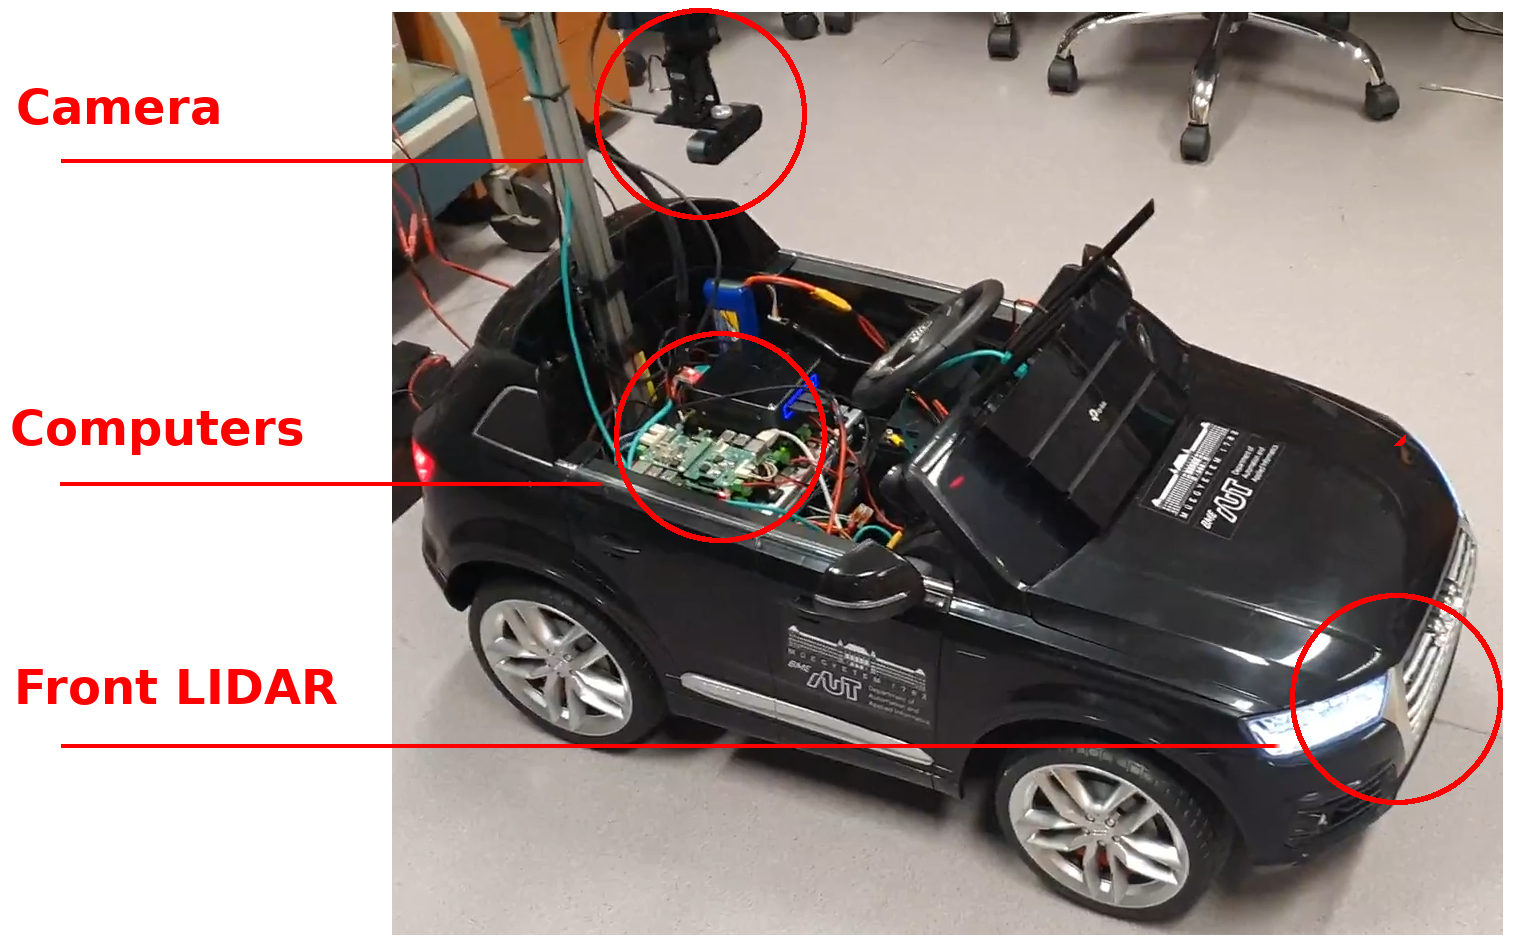
\includegraphics[height=80mm]{figures/raw/car_setup_front.png}
    \caption{The car setup (front side)}
    \label{car_setup_front}
\end{figure}

Amongst others, the car is equipped with a front, a rear and a top LIDAR, a camera, inertial sensors, ultrasonic distance sensors, several Raspberry Pi-s and an Intel NUC computer.

\begin{figure}[!ht]
    \centering
    \includegraphics[height=100mm]{figures/raw/car_setup_rear.png}
    \caption{The car setup (rear side)}
    \label{car_setup_rear}
\end{figure}

The vehicle supports the development and testing of multiple smaller projects (mapping and navigation algorithms, control modules, etc.), all contributing to the car becoming more and more able to drive itself. For these sub-projects, the above mentioned sensors are all needed, later I will explain them in detail. These sensors and computers provide a good hardware base for the project, but they are not all that's necessary. A project of this complexity cannot be maintained without a reliable and robust software framework to build upon. This framework is ROS.

\subsection{About ROS}

\begin{quote}
The Robot Operating System (ROS) is a \textbf{set of software libraries} and tools that help you build robot applications. From drivers to state-of-the-art algorithms, and with powerful developer tools, ROS has what you need for your next robotics project. And it's all \textbf{open source}.
\end{quote}

The above description is quoted from their \href{https://www.ros.org/}{website}. Short as it may be, their description does point out that ROS is a software framework for robotic applications. Wikipedia also has a brief and comprehensible \href{https://en.wikipedia.org/wiki/Robot_Operating_System}{article} about ROS, in which it states that:

\begin{quote}
Although ROS is \textbf{not an operating system}, it provides services designed for a heterogeneous computer cluster such as hardware abstraction, low-level device control, implementation of commonly used functionality, message-passing between processes, and package management. Running sets of ROS-based processes are represented in a \textbf{graph architecture} where processing takes place in nodes that may receive, post and multiplex sensor data, control, state, planning, actuator, and other messages. Despite the importance of reactivity and low latency in robot control, ROS itself is not a real-time OS (RTOS). It is possible, however, to integrate ROS with real-time code.
\end{quote}

So what is ROS exactly? It is a framework that helps building robot applications. It is basically a large set of software components with an own build system. It is not an operating system, therefore it needs one under it. Although it may be installed on Debian and Windows 10 as well, its main target OS is Ubuntu. For this reason, the chosen OS for the computers in the project became Ubuntu (versions Artful and Bionic are supported).

All ROS applications have a graph architecture, meaning that they are considered as a set of separate processes (nodes) that are connected via messages. The standard defines some popular message types, but supports custom messages as well. The communication through messages is based on the publish-subscribe model, a publisher provides some data in the form of messages that all subscribed nodes can read. The implementation of the message-passing, the used networks layer and the transmission and reception of the messages are hidden from the application. ROS handles the delivery between different processes and even different hosts.

What ROS guarantees is a stable build system and architecture that helps developers create multi-process applications relatively easy, with reliable message-passing over a configurable transport layer (TCP by default). However, these features would not be enough for developers to consider ROS a relevant candidate for a robotic application framework, easy-to-integrate tools and a detailed documentation are also necessary. Fortunately, ROS does include these.

Its documentation is comprehensible and covers most topics that developers may need to look into. Besides that, a large series of tutorials are also available on their website about getting started with ROS and building simple applications, and also about deeper topics that give major insight to the reader about how ROS tools and features can be used effectively. These tutorials usually demonstrate given features using example applications that are also available for installing.

\subsection{Useful ROS tools}
ROS comes with numerous tools that are plug-and-play compatible any applications, due to that fact that ROS apps are just a set of independent nodes - once opened, these tools become nodes in the ROS graph and they can communicate with the other nodes via messages.

One of most essential tool is \href{http://wiki.ros.org/rviz}{rviz}, a 3D visualization tool. rviz supports a wide range of elements that it can display (camera images, maps, markers, point clouds, robot models, etc.), and the developers also have the option to implement custom display plugins for their own types.

\begin{figure}[!ht]
	\centering
	\includegraphics[width=\textwidth]{figures/raw/rviz.png}
	\caption{rviz}
	\label{rviz}
\end{figure}

For vehicle applications such as the \textit{vr-car} project, the typical displayed types are robot models, odometry, trajectories and maps. Just imagining the simplest car driving project we can, displaying the car's position and orientation could be quite useful. Unsurprisingly, rviz supports the visualization of vehicle odometry (see \href{http://wiki.ros.org/rviz/DisplayTypes/Odometry}{Odometry display type}), and according to its documentation:

\begin{quote}
	The Odometry display accumulates a \href{http://docs.ros.org/api/nav_msgs/html/msg/Odometry.html}{nav\_msgs/Odometry} message over time, showing them as arrows.
\end{quote}

So one of the nodes in the project's graph needs to publish the odometry messages, and no further coding is needed, rviz may be opened and odometry will be displayed.

Another useful program is \href{http://gazebosim.org/}{Gazebo}, which is an open-source 3D robotics simulator that can be connected to ROS easily.

In the next sections I am going to explain the ROS graph and the message-passing between nodes using a simplified model of the \textit{vr-car} project, while also describing the features of the application and most useful developer tools provided by ROS.

\subsection{Remote drive}
The first (and probably simplest to comprehend) feature of the car is the ability to control it remotely, using either a PC keyboard, a joystick or a set of racing wheel and pedals.

In order to make this possible, the car definitely needs a node that controls the car's actuators according to an input actuation. For simplicity, let's assume that this input actuation (a ROS message) contains a target speed and wheel angle that the module has to handle as a reference. Having direct control of the car's motors (the accelerator DC motor and the steering servo) and of the necessary sensors (e.g. a rotary encoder for measuring speed) the control is manageable.

Besides this control module, the graph must contain another node, that reads driver interactions (key strokes, joystick state or steering wheel and pedal positions), converts these to driver commands (target actuations) and publishes the correspondent messages that the control node listens to. Note, that these input nodes are implemented separately for the input types - there is a module for keyboard input, one for handling the joystick and a third one for reading the racing wheel and pedal data\footnote{The racing wheel and the throttle and brake pedals are actually handled on a separate Windows host, and their positions are forwarded to another host running ROS.}.

\tikzset{
	base_node/.style    = {rectangle, rounded corners, draw=black,
		minimum width=4.5cm, minimum height=1cm,
		text centered, font=\sffamily},
	common_node/.style  = {base_node, fill=orange!15},
	decoration={brace},
	tuborg/.style={decorate},
	tubnode_left/.style={midway, left=2pt},
	tubnode_right/.style={midway, right=2pt}
}

\begin{figure}[!ht]
	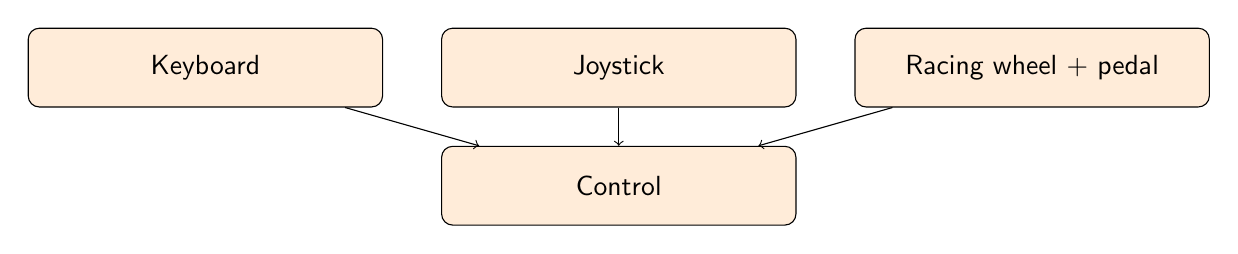
\begin{tikzpicture}[
	node distance=1.5cm,
	every node/.style={fill=white, font=\sffamily}, align=center]
	% Input nodes
	\node (input_keyboard)    [common_node]                          {Keyboard};
	\node (input_joystick)    [common_node, xshift=5.25cm]           {Joystick};
	\node (input_wheel_pedal) [common_node, xshift=10.5cm]           {Racing wheel + pedal};
	% Control node
	\node (control)           [common_node, below of=input_joystick] {Control};
	% Connections
	\draw[->]    (input_keyboard) -- (control);
	\draw[->]    (input_joystick) -- (control);
	\draw[->] (input_wheel_pedal) -- (control);
	\end{tikzpicture}
	\caption{Remote drive}
	\label{remote_drive}
\end{figure}

With one input module being active, the graph now contains two processes - the input and the control nodes. These two nodes are communicating through a message that contains speed and wheel angle reference values. The setup may be called finished, as it is working. However, ROS provides tools that take little amount of code to incorporate, but prove to be very useful.

\subsection{\textit{vr-drive}}

